\section{Versuchsaufbau}

\fbox{\parbox{\textwidth}{
\noindent\textbf{Inhalt}
\begin{itemize}
    \item Simulierte Datensätze
        \begin{itemize}
            \item Einzelne Datensätze (Kugeln, Kugeln mit andere Dichte, Zylinder, Quader)
            \item Gemischte Datensätze
        \end{itemize}
    \item Realdaten
\end{itemize}
}}

\begin{figure}[!h]
    \centering
    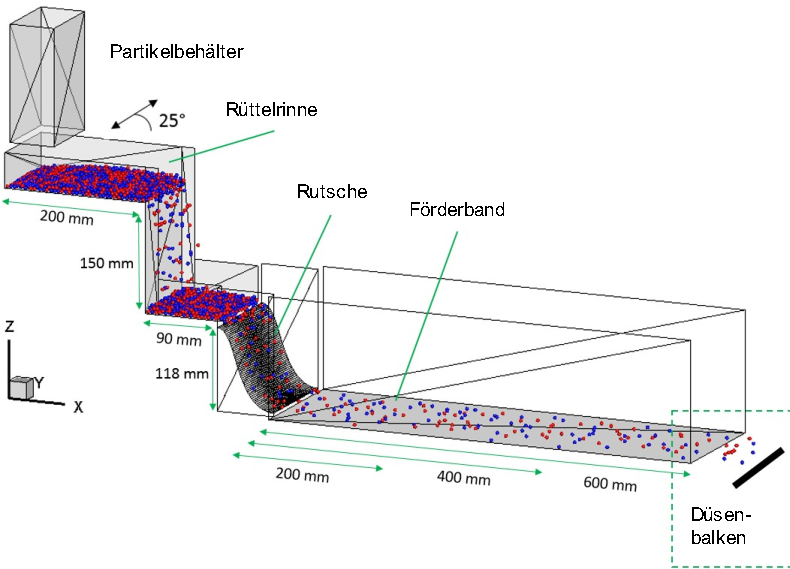
\includegraphics[width=0.7\textwidth]{pics/SimulationsAufbau.pdf}
    \caption{Aufbau \cite{ITM07_BrunnSawo}}
    \label{fig:SimAufbau}
\end{figure}